\documentclass{article}
\usepackage{graphicx} 
\usepackage[colorlinks=true, linkcolor=blue, urlcolor=red]{hyperref}
\usepackage[utf8]{inputenc}
\usepackage[T1]{fontenc}
\usepackage{lmodern} 
\usepackage[polish]{babel}
\usepackage{float} 
\usepackage{listings}
\usepackage{xcolor}
\usepackage{amsmath}

\lstnewenvironment{Rcode}[1][]{
    \lstset{
        language=R,
        basicstyle=\ttfamily,
        keywordstyle=\color{blue},
        commentstyle=\color{green!40!black},
        stringstyle=\color{orange},
        showstringspaces=false,
        frame=single,
        numbers=left,
        numberstyle=\tiny,
        numbersep=5pt,
        breaklines=true,
        #1
    }
}{}

\title{Statystyka Wielowymiarowa}
\author{Adam Staniszewski}
\date{May 2024}

\begin{document}

\maketitle

\tableofcontents  % Add table of contents here

\section{Dobór zbioru danych}
Do wykonywania zadań został wybrany zbiór \href{https://www.kaggle.com/datasets/girumwondemagegn/dataset-for-renewable-energy-systems}{Dataset for renewable energy systems}. Składa się on z 13 kolumn i około 15000 wierszy. 

Dodatkowo, dla zadań klasyfikacji binarnej, kolumna \textbf{Type\_of\_Renewable\_Energy} została przerobiona na 7 osobnych kolumn, reprezentujących źródła energii:
\begin{itemize}
    \item \textbf{Solar},
    \item \textbf{Wind},
    \item \textbf{Hydroelectric},
    \item \textbf{Geothermal},
    \item \textbf{Biomass},
    \item \textbf{Tidal},
    \item \textbf{Wave},
\end{itemize}

\section{Laboratorium 1}
\subsection{Regresja liniowa}
Na początku przeprowadzamy prostą regresję liniową:

\begin{figure}[H]
    \centering
    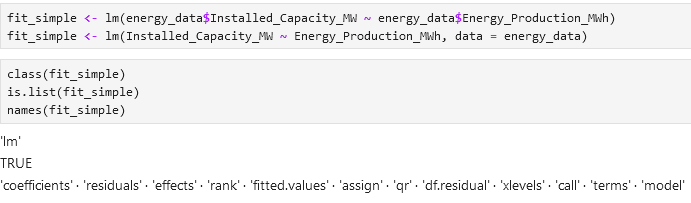
\includegraphics[width=0.9\linewidth]{lab1/obraz.png}
    \caption{Zmienna objaśniana - Installed Capacity MW. Zmienna objaśniająca - Energy Production MWh}
    \label{fig:regression}
\end{figure}

\begin{figure}[H]
    \centering
    \includegraphics[width=0.9\linewidth]{lab1/obraz2.png}
    \caption{Współczynniki regresji}
    \label{fig:coefficients}
\end{figure}

\begin{figure}[H]
    \centering
    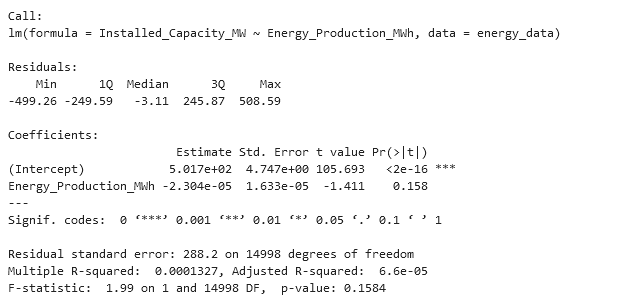
\includegraphics[width=0.9\linewidth]{lab1/obraz3.png}
    \caption{Podsumowanie regresji liniowej}
    \label{fig:summary}
\end{figure}

\begin{figure}[H]
    \centering
    \includegraphics[width=0.9\linewidth]{lab1/obraz4.png}
    \caption{Wartości rzeczywiste vs przewidywane}
    \label{fig:real_vs_predicted}
\end{figure}

\begin{figure}[H]
    \centering
    \includegraphics[width=0.9\linewidth]{lab1/obraz5.png}
    \caption{Reszty regresji}
    \label{fig:residuals}
\end{figure}

\begin{figure}[H]
    \centering
    \includegraphics[width=0.9\linewidth]{lab1/obraz6.png}
    \caption{Heat values}
    \label{fig:heat_values}
\end{figure}

\subsection{Regresja wielokrotna}
Przejdźmy do regresji wielokrotnej. Będziemy przewidywać wartość \textbf{Installed\_Capacity\_MW} na podstawie zmiennych \textbf{Energy\_Production\_MWh} i \textbf{Energy\_Consumption\_MWh}.

\begin{Rcode}
fit_la <- lm(energy_data$Installed_Capacity_MW ~ energy_data$Energy_Production_MWh + energy_data$Energy_Consumption_MWh)
\end{Rcode}

\begin{figure}[H]
    \centering
    \includegraphics[width=1\linewidth]{lab1/obraz9.png}
    \caption{Enter Caption}
    \label{fig:enter-label}
\end{figure}

Przeprowadźmy teraz regresję wielokrotną dla jednej zmiennej dla pozostałych zmiennych liczbowych:

\begin{Rcode}
numerical_data <- energy_data[, sapply(energy_data, is.numeric)]
fit_all <- lm(Installed_Capacity_MW ~ ., data = numerical_data)
\end{Rcode}

\begin{figure}[H]
    \centering
    \includegraphics[width=1\linewidth]{lab1/obraz10.png}
    \caption{Enter Caption}
    \label{fig:enter-label}
\end{figure}

\begin{figure}[H]
    \centering
    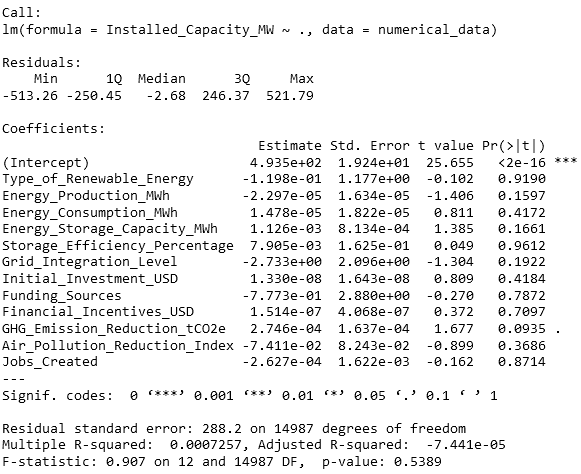
\includegraphics[width=1\linewidth]{lab1/obraz11.png}
    \caption{Enter Caption}
    \label{fig:enter-label}
\end{figure}

A teraz bez zmiennej Grid\_Integration\_Level:

\begin{Rcode}
fit_no_grid_int <- update(fit_all, ~ . - Grid_Integration_Level)
summary(fit_no_grid_int)
\end{Rcode}

\begin{figure}[H]
    \centering
    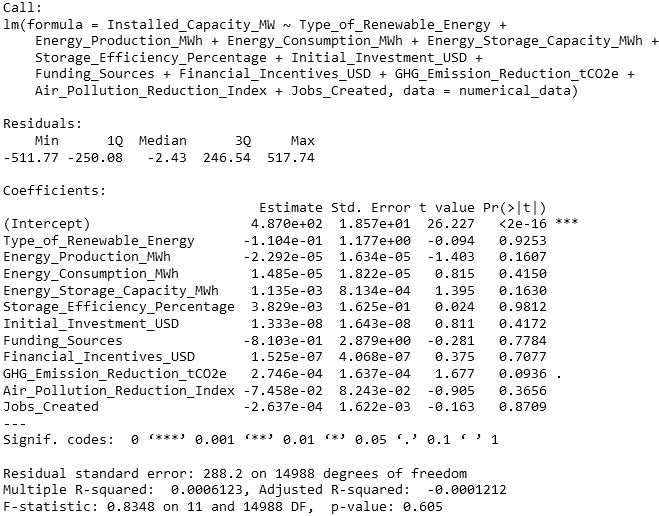
\includegraphics[width=1\linewidth]{lab1/obraz12.png}
    \caption{Enter Caption}
    \label{fig:enter-label}
\end{figure}

Wybrane przedziały ufności:

\begin{figure}[H]
    \centering
    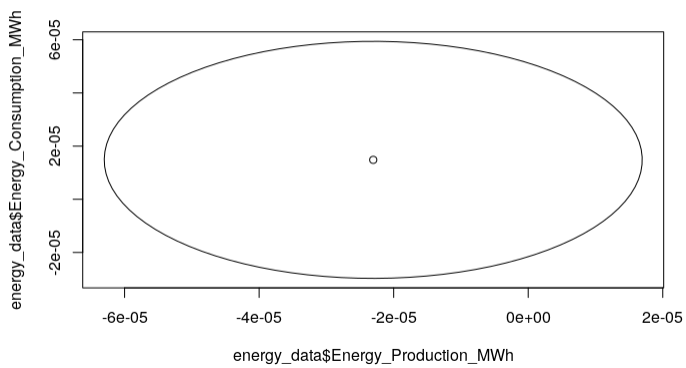
\includegraphics[width=1\linewidth]{lab1/obraz13.png}
    \caption{Enter Caption}
    \label{fig:enter-label}
\end{figure}

Sprawdźmy jeszcze jak poradzi sobie regresja wielomianowa (5 stopnia):

\begin{Rcode}
anova(fit_simple, fit_l2)
fit_l5 <- lm(energy_data$Energy_Consumption_MWh ~ poly(energy_data$Energy_Production_MWh, 5))
summary(fit_l5)
summary(lm(Energy_Production_MWh ~ log(Energy_Consumption_MWh), data = energy_data))
\end{Rcode}

\begin{figure}[H]
    \centering
    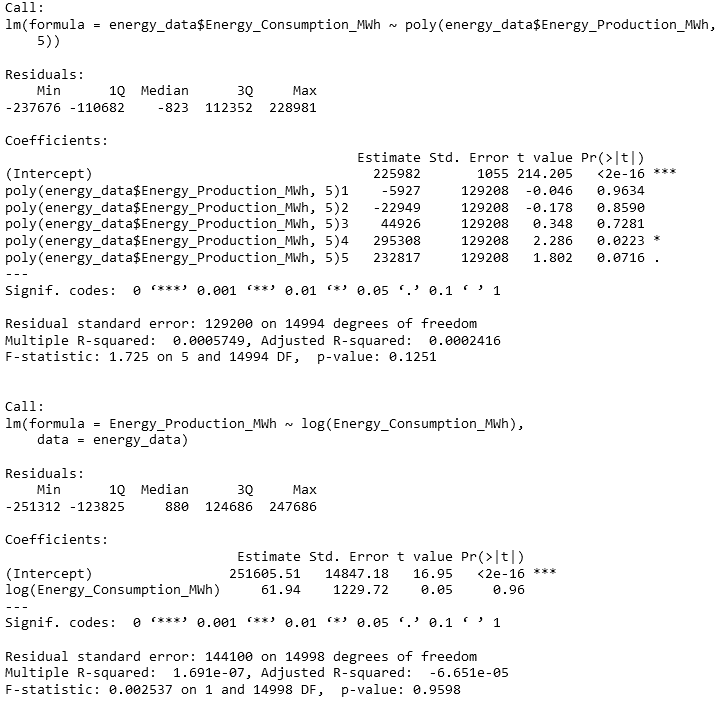
\includegraphics[width=1\linewidth]{lab1/obraz14.png}
    \caption{Enter Caption}
    \label{fig:enter-label}
\end{figure}

\section{Laboratorium 2}
\subsection{One hot encoding i korelacje}
Jak wspomniano we wstępie, dla zadań klayfikacji binarnej wykonany został \textbf{One Hot Encoding} kolumny \textbf{Type\_Of\_Renewable\_Energy}. Ze względu na problemy ze środowiskiem wykonawczym, odpowiednia funkcja została napisana bez użycia zewnętrznych bibliotek:

\begin{Rcode}
unique_types <- unique(energy_data$Type_of_Renewable_Energy)

for (type in unique_types) {
  column_name <- paste("Type_of_Renewable_Energy", type, sep = "_")
  energy_data[[column_name]] <- ifelse(energy_data$Type_of_Renewable_Energy == type, 1, 0)
}

energy_data <- subset(energy_data, select = -c(Type_of_Renewable_Energy))
\end{Rcode}

Otrzymujemy w ten sposób 7 dodatkowych kolumn o binarnych wartościach, które zostaną użyte jako cel klasyfikacji.

Znajdźmy najsilniejsze korelacje między cechami (pomijając korelacje między tymi samymi cechami):

\begin{Rcode}
numeric_data <- energy_data[sapply(energy_data, is.numeric)]
corr_mat <- cor(numeric_data)
corr_df <- as.data.frame(as.table(corr_mat))
corr_df <- corr_df[corr_df$Var1 != corr_df$Var2,]
corr_df <- corr_df[order(abs(corr_df$Freq)),]
top_corrs <- head(corr_df, 10)
\end{Rcode}

\begin{figure}[H]
    \centering
    \includegraphics[width=1\linewidth]{lab2/obraz.png}
    \caption{Zmienne o najwyższych korelacjach.}
    \label{fig:enter-label}
\end{figure}

\subsection{Regresja logistyczna}

Spróbujmy przywidzieć czy dane źródło energii należy do \textbf{1 kategorii} za pomocą zmiennych \textbf{Installed\_Capacity\_MW}, \textbf{Energy\_Production\_MWh}, \textbf{Energy\_Storage\_Capacity\_MWh} i \textbf{Storage\_Efficiency\_Percentage}.

\begin{Rcode}
dir_logistic <- list()
dir_logistic$fit <- glm(Type_of_Renewable_Energy_1 ~ Installed_Capacity_MW + Energy_Production_MWh 
                        + Energy_Storage_Capacity_MWh + Storage_Efficiency_Percentage, 
                   family = binomial, data = energy_data)
dir_logistic$predicted <- ifelse(dir_logistic$probs > 0.5, "Type 1", "Not type 1")
dir_logistic$cm <- table(dir_logistic$predicted, energy_data$Type_of_Renewable_Energy_1)
dir_logistic$cm
\end{Rcode}

Otrzymujemy wyniki:
\begin{figure}[H]
    \centering
    \includegraphics[width=0.7\linewidth]{lab2/obraz3.png}
    \caption{Nienależność i należność do badanej klasy}
    \label{fig:enter-label}
\end{figure}

Finalnie otrzymaliśmy proporcję błędów treningowych równą 0 - być może zadanie jest zbyt trywialne. Sprawdźmy jak wyniki zmieni poprawny podział zbioru.

\subsection{Podział zbioru}
Losowo dzielimy zbiór na treningowy i testowy w proporcjach 70/30:

\begin{Rcode}
set.seed(123)

train_indices <- sample(nrow(energy_data), round(0.7 * nrow(energy_data)))
train <- energy_data[train_indices, ]
energy_data_test <- energy_data[-train_indices, ]
Type_of_Renewable_Energy_1_test <- energy_data_test$Type_of_Renewable_Energy_1
\end{Rcode}

Wykonujemy regresję na zbiorze treningowym:

\begin{Rcode}
dir_log_t <- list()
dir_log_t$fit <- glm(Type_of_Renewable_Energy_1 ~ Installed_Capacity_MW + Energy_Production_MWh, 
                   family = binomial, data = train)
\end{Rcode}

\begin{figure}[H]
    \centering
    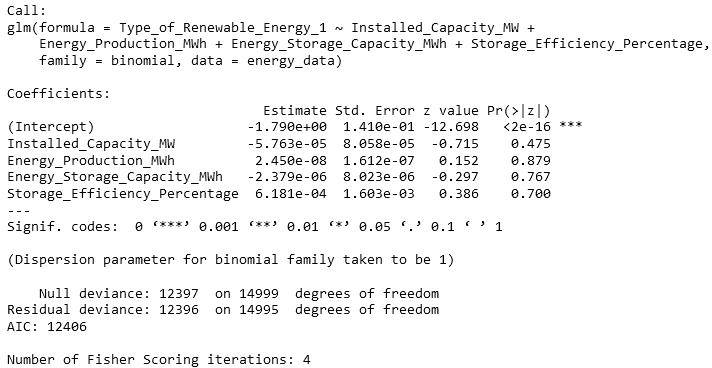
\includegraphics[width=1\linewidth]{lab2/obraz4.png}
    \caption{Podsumowanie regresji na zbiorze treningowym.}
    \label{fig:enter-label}
\end{figure}

Sprawdźmy predykcje na zbiorze testowym:

\begin{Rcode}
dir_log_t$probs <- predict(dir_log_t$fit, energy_data_test, type = "response")
dir_log_t$predicted <- ifelse(dir_log_t$probs > 0.5, "Type 1", "Not type 1")
table(dir_log_t$predicted, Type_of_Renewable_Energy_1_test)
\end{Rcode}

\begin{figure}[H]
    \centering
    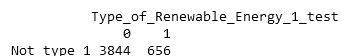
\includegraphics[width=0.75\linewidth]{lab2/obraz5.png}
    \caption{Macierz pomyłek}
    \label{fig:enter-label}
\end{figure}

W tym przypadku otrzymaliśmy proprocję błędów na poziomie około 20\%.

Użyjmy predyktorów mocniej skorelowanych ze zmienną objaśnianą, czyli \textbf{Energy\_Production\_MWh} i \textbf{Energy\_Storage\_Capacity\_MWh}:

\begin{Rcode}
dir_log_best2$fit <- glm(Type_of_Renewable_Energy_1 ~ Installed_Capacity_MW + Energy_Production_MWh, 
                         family = binomial, 
                    data = energy_data, subset = train)
summary(dir_log_best2$fit)
dir_log_best2$probs <- predict(dir_log_best2$fit, energy_data_test, type = "response")
dir_log_best2$predicted <- ifelse(dir_log_best2$probs > 0.5, "Type 1", "Not type 1")
table(dir_log_best2$predicted, Type_of_Renewable_Energy_1_test)
\end{Rcode}

\subsection{Metoda LDA}
Dokonajmy ponownego podziału na potrzeby kolejnych metod klasyfikacji:
\begin{Rcode}
set.seed(123) 
train_indices <- sample(1:nrow(energy_data), 0.7 * nrow(energy_data))
train <- rep(FALSE, nrow(energy_data))
train[train_indices] <- TRUE

test <- !train
test <- energy_data[test, ]
\end{Rcode}

Przeprowadzamy \textbf{LDA} wraz z obliczeniem proporcji błędów na zbiorze testowym:
\begin{Rcode}
dir_lda <- list()
dir_lda$fit <- lda(Type_of_Renewable_Energy_1 ~ Energy_Production_MWh + Energy_Storage_Capacity_MWh, data = energy_data, subset = train)

print(dir_lda$fit)

dir_lda$predicted <- predict(dir_lda$fit, test)
predicted_classes <- dir_lda$predicted$class
actual_classes <- test$Type_of_Renewable_Energy_1
num_errors <- sum(predicted_classes != actual_classes)

total_samples <- length(actual_classes)
proportion_of_errors <- num_errors / total_samples

print(proportion_of_errors)
\end{Rcode}

Podsumowanie LDA:
\begin{figure}[H]
    \centering
    \includegraphics[width=1\linewidth]{lab2/obraz6.png}
    \caption{Podsumowanie LDA}
    \label{fig:enter-label}
\end{figure}

Prawdopodobieństwo przynależności do klasy wynosi około 14.4\%. Jeśli weźmiemy pod uwagę, że mamy 7 możliwych klas, to będziemy w stanie wywnioskować, że zbiór jest zbalansowany pod względem ich liczności.

Proporcja błędu to z kolei około 14.6\% - lepiej niż przy regresji logistycznej.

\subsection{Metoda QDA}
Przeprowadźmy analogiczną analizę przy pomocy \textbf{QDA}:

\begin{Rcode}
dir_qda <- list()
dir_qda$fit <- qda(Type_of_Renewable_Energy_1 ~ Energy_Production_MWh + Energy_Storage_Capacity_MWh, data = energy_data, subset = train)

print(dir_qda$fit)

dir_qda$predicted <- predict(dir_qda$fit, test)
predicted_classes <- dir_qda$predicted$class

actual_classes <- test$Type_of_Renewable_Energy_1
num_errors <- sum(predicted_classes != actual_classes)
total_samples <- length(actual_classes)

proportion_of_errors <- num_errors / total_samples
print(proportion_of_errors)
\end{Rcode}

\begin{figure}[H]
    \centering
    \includegraphics[width=1\linewidth]{lab2/obraz7.png}
    \caption{Podsumowanie QDA}
    \label{fig:enter-label}
\end{figure}

Proporcja błędów jest w tym przypadku taka sama, jak w LDA.

\subsection{Metoda kNN}
Na koniec sprawdźmy wyniki dla metody \textbf{kNN}, dla różnych wartości parametru \textbf{k}. W tym przypadku lekko modyfikujemy zbiory:

\begin{Rcode}
train_set <- energy_data[train, c("Energy_Storage_Capacity_MWh", "Energy_Production_MWh")]
test_set <- energy_data[!train, c("Energy_Storage_Capacity_MWh", "Energy_Production_MWh")]
renewable_energy_train <- energy_data$Type_of_Renewable_Energy_1[train]
Type_of_Renewable_Energy_1_test <- energy_data$Type_of_Renewable_Energy_1[!train]  
\end{Rcode}

Używamy kNN w pętli:
\begin{Rcode}
dir_knn <- knn(train_set, test_set, renewable_energy_train, k = k)
num_errors <- sum(dir_knn != Type_of_Renewable_Energy_1_test)
total_samples <- length(Type_of_Renewable_Energy_1_test)
\end{Rcode}

Zależność proporcji błędu od ilości parametrów:

\begin{figure}[H]
    \centering
    \includegraphics[width=1\linewidth]{lab2/obraz8.png}
    \caption{Wyniki dla kNN}
    \label{fig:enter-label}
\end{figure}

Dla \( k \geq 2 \) widzimy wartości wyższe lub zbliżone do regresji logistycznej. Dla wartości \( k \leq 8 \) wartości są najlepsze ze wszystkich metod.



\section{Laboratorium 3}
\subsection{Walidacja krzyżowa}
\subsubsection{Metoda zbioru walidacyjnego}
Na początku wczytuję dane, usuwam wartości NaN i przygotowuję zbiór walidacyjny.

\begin{Rcode}
energy_data <- read.csv("energy_dataset.csv")
energy_data <- na.omit(energy_data)
set.seed(1)
n <- nrow(energy_data)
train <- sample(n, n / 2)
\end{Rcode}
Dopasowuję model liniowy na zbiorze uczącym i obliczam MSE dla zbioru walidacyjnego:

\begin{Rcode}
energy_lm <- lm(Type_of_Renewable_Energy ~ Energy_Production_MWh,
                 data = energy_data,
                 subset = train)

validation_set <- energy_data[-train,]

mse <- mean((validation_set$Type_of_Renewable_Energy -
              predict(energy_lm, validation_set))^2)

\end{Rcode}
Otrzymana wartość MSE: \textbf{4.0439057662439}.

Użyjmy wielomianów o różnych stopniach:

\end{Rcode}
Dopasowuję model liniowy na zbiorze uczącym i obliczam MSE dla zbioru walidacyjnego:

\begin{Rcode}
for (i in 2:5) {
  energy_lm_poly <- lm(Type_of_Renewable_Energy ~ poly(Energy_Production_MWh, degree = i), data = energy_data, 
                     subset = train)
  print(mean((validation_set$Type_of_Renewable_Energy - predict(energy_lm_poly, validation_set))^2))
}
\end{Rcode}
Otrzymujemy MSE: 

\begin{Rcode}
[1] 4.042959
[1] 4.041494
[1] 4.041374
[1] 4.042979
\end{Rcode}
\textbf{Wniosek} - stopień wielomianu w tym przypadku nie ma znaczącego wpływu na otrzymany MSE.
Powtarzam obliczenia dla innego zbioru walidacyjnego:

\begin{Rcode}
degree_max <- 5

compute_mse <- function(degree, train) {
  energy_lm <- lm(Type_of_Renewable_Energy ~ poly(Energy_Production_MWh, degree), data = energy_data, subset = train)
  validation_set <- energy_data[-train,]
  mean((validation_set$Type_of_Renewable_Energy - predict(energy_lm, validation_set))^2)
}

mse <- vapply(1:degree_max, compute_mse, FUN.VALUE = numeric(1), train = train)
\end{Rcode}
Otrzymane wartości MSE:
\begin{Rcode}
4.04390576624393
4.04295881295649
4.04149420436449
4.04137383913034
4.04297885010734
\end{Rcode}

\begin{figure}[H]
    \centering
    \includegraphics[width=0.8\linewidth]{lab3/obraz.png}
    \caption{Zależność między wartością MSE a stopniem wielomianu.}
    \label{fig:enter-label}
\end{figure}

\subsubsection{Walidacja krzyżowa bez jednego (leave-one-out)}

\begin{Rcode}
set.seed(2)
train <- sample(n, n / 2)
validation_set <- energy_data[-train,]
degree_max <- 10
mse <- rep(0, times = degree_max)
for (i in 1:degree_max) {
  energy_lm <- lm(Type_of_Renewable_Energy ~ poly(Energy_Production_MWh, degree = i), data = energy_data, subset = train)
  mse[i] <- mean((validation_set$Type_of_Renewable_Energy - predict(energy_lm, validation_set))^2)
}
mse
\end{Rcode}

\begin{Rcode}
    TUTAJ WYKRES TEGO WYZEJ
\end{Rcode}

\begin{Rcode}
[Co teraz z wnioskami na temat regresji wielomianowej w naszym przypadku?]
[Sprawdź, że dla LOOCV obie współrzędne delta zawierają praktycznie to samo.]
\end{Rcode}

\subsubsection{K-krotna walidacja krzyżowa}
Tym razem jawnie ustawiamy parametr K oznaczający liczbę grup:

\begin{Rcode}
compute_kcv_mse <- function(degree, k) {
    energy_glm <- glm(Type_of_Renewable_Energy ~ poly(Energy_Production_MWh, degree), data = energy_data)
    cv.glm(energy_data, energy_glm, K = k)$delta[1]
}
mse <- sapply(1:degree_max, compute_kcv_mse, k = 10)
\end{Rcode}
Zestawiamy 10 wyników:
\begin{Rcode}
mse10 <- replicate(10, sapply(1:degree_max, compute_kcv_mse, k = 10))
\end{Rcode}
Otrzymujemy:
\begin{Rcode}
    10 WYNIKOW
\end{Rcode}
\begin{Rcode}
    WYKRES
\end{Rcode}
\begin{Rcode}
    CO Z WYNIKAMI
\end{Rcode}

\subsubsection{Bootstrap}
Użyjmy metody bootstrap do oszacowania błędów standardowych współczynników regresji liniowej.

\begin{Rcode}
lm_coefs <- function(data, index = 1:nrow(data)) {
  coef(lm(Type_of_Renewable_Energy ~ Energy_Production_MWh, data = energy_data, subset = index))
}

n <- nrow(energy_data)
lm_coefs(energy_data, sample(n, n, replace = TRUE))

lm_coefs(energy_data)

boot(energy_data, lm_coefs, R = 1000)
}
\end{Rcode}

W ten sposób obliczyliśmy błąd standardowy z 1000 replikacji.

\begin{figure}[H]
    \centering
    \includegraphics[width=1\linewidth]{lab3/obraz2.png}
    \caption{Wyniki dla regresji liniowej z użyciem metody boostrap}
    \label{fig:enter-label}
\end{figure}

Powtórzmy eksperyment dla regresji kwadratowej:

\begin{Rcode}
lm_coefs <- function(data, index = 1:nrow(data)) {
  coef(lm(Type_of_Renewable_Energy ~ (Energy_Production_MWh)^2, data = energy_data, subset = index))
}

n <- nrow(energy_data)
lm_coefs(energy_data, sample(n, n, replace = TRUE))

lm_coefs(energy_data)

boot(energy_data, lm_coefs, R = 1000)
\end{Rcode}

\begin{figure}[H]
    \centering
    \includegraphics[width=1\linewidth]{lab3/obraz2_5.png}
    \caption{Wyniki dla regresji kwadratowej z użyciem metody boostrap}
    \label{fig:enter-label}
\end{figure}

\subsection{Selekcja cech dla modeli liniowych}
Podzielmy nasz główny zbiór na podzbiory za pomocą metody \textit{regsubsets}. Wykorzystamy wszystkie 12 zmiennych objaśniających

\begin{Rcode}
energy_bs <- regsubsets(Type_of_Renewable_Energy ~ ., data = energy_data, nvmax=12)
energy_bs_sum <- summary(energy_bs)
energy_bs_sum
\end{Rcode}

Sprawdźmy, który predyktor zagwarantuje mam najlepszy podzbiór. Używamy metryki \textbf{BIC}, która powinna być jak najmniejsza.

\begin{Rcode}
energy_bs_sum$cp
bic_min <- which.min(energy_bs_sum$bic)
bic_min
energy_bs_sum$bic[bic_min]

energy_bs_sum

plot(energy_bs_sum$bic, xlab = "Liczba zmiennych", ylab = "BIC", col = "green",
     type = "b", pch = 20)
points(bic_min, energy_bs_sum$bic[bic_min], col = "red", pch = 9)

plot(energy_bs, scale = "bic")    
\end{Rcode}

\begin{figure}[H]
    \centering
    \includegraphics[width=1\linewidth]{lab3/obraz3_5.png}
    \caption{Liczba zmiennych a wartość BIC}
    \label{fig:enter-label}
\end{figure}

\begin{figure}[H]
    \centering
    \includegraphics[width=1\linewidth]{lab3/obraz3.png}
    \caption{Ocena predyktorów}
    \label{fig:enter-label}
\end{figure}

Najlepszym wyborem zdaje się być \textbf{grid\_integration\_level}.

Estymaty parametrów dla optymalnego podzbioru:

\begin{Rcode}
coef(energy_bs, id = 8)
\end{Rcode}

\begin{figure}[H]
    \centering
    \includegraphics[width=1\linewidth]{lab3/obraz4.png}
    \caption{Podusmowanie dla metryki BIC}
    \label{fig:enter-label}
\end{figure}

Wykorzystajmy jeszcze metrykę \textbf{$R^2$}, zaimplementowaną analogicznie do BIC.

\begin{figure}[H]
    \centering
    \includegraphics[width=1\linewidth]{lab3/obraz6.png}
    \caption{Liczba zmiennych a wartość $R^2$}
    \label{fig:enter-label}
\end{figure}

\begin{figure}[H]
    \centering
    \includegraphics[width=1\linewidth]{lab3/obraz7.png}
    \caption{Ocena predyktorów}
    \label{fig:enter-label}
\end{figure}

Według metryki $R^2$, najlepszymi predyktorami są \textbf{Initial\_Investment\_USD} i \textbf{GHG\_Emission\_Reduction\_tCO2e}.

\subsubsection{Selekcja krokowa do przodu i wstecz}
Używamy teraz selekcji krokowej

\begin{Rcode}
energy_fwd <- regsubsets(Type_of_Renewable_Energy ~ ., data = energy_data, nvmax=10, 
                          method = "forward")
energy_fwd_sum <- summary(energy_fwd)
energy_fwd_sum
energy_back <- regsubsets(Type_of_Renewable_Energy ~ ., data = energy_data, nvmax=10, 
                          method = "backward")
energy_back_sum <- summary(energy_back)
energy_back_sum
\end{Rcode}

\begin{figure}[H]
    \centering
    \includegraphics[width=1\linewidth]{lab3/obraz5.png}
    \caption{Enter Caption}
    \label{fig:enter-label}
\end{figure}

\subsubsection{Wybór modelu przy pomocy metody zbioru walidacyjnego}

\begin{Rcode}
n <- nrow(energy_data)
train <- sample(c(TRUE, FALSE), n, replace = TRUE)
test <- !train
energy_bs_v <- regsubsets(Type_of_Renewable_Energy ~ ., data = energy_data, nvmax=10)
\end{Rcode}

\begin{Rcode}
predict.regsubsets <- function(object, newdata, id, ...) {
  model_formula <- as.formula(object$call[[2]])
  mat <- model.matrix(model_formula, newdata)
  coefs <- coef(object, id = id)
  mat[, names(coefs)] %*% coefs
}
\end{Rcode}

\begin{Rcode}
prediction_error <- function(i, model, subset) {
pred <- predict(model, energy_data[subset,], id = i)
mean((energy_data$Type_of_Renewable_Energy[subset] - pred)^2)
}
val_errors <- sapply(1:10, prediction_error, model = energy_bs_v, subset = test)
val_errors   
\end{Rcode}

Otrzymaliśmy takie wartości błędu: 
\begin{Rcode}
4.013148 4.012435 4.012165 4.011892 4.011292 4.011261 4.011174 4.010870 4.010838 4.010614
\end{Rcode}
Możemy więc wywnioskować, że optymalny model ma 10 parametrów.

\subsubsection{Wybór modelu przy pomocy k-krotnej walidacji krzyżowej}

\begin{Rcode}
k <- 10
folds <- sample(1:k, n, replace = TRUE)
val_err <- NULL
for (j in 1:k) {
  fit_bs <- regsubsets(Type_of_Renewable_Energy ~ ., data = energy_data[folds != j,], nvmax=10)
  err <- sapply(1:10, prediction_error, model = fit_bs, subset = (folds == j))
  val_err <- rbind(val_err, err)
}

cv_errors <- colMeans(val_err)
cv_errors
\end{Rcode}

Otrzymaliśmy takie wartości błędów:

\begin{Rcode}
3.998710 3.996294 3.998936 3.999858 4.000146 4.000639 4.000911 4.000728 4.000925 4.000906
\end{Rcode}

Według tego kryterium, optymalny model powinien mieć dwa parametry.

\section{Laboratorium 4}
\subsection{Regularyzacja}
Zajmijmy się regularyzacją naszego zbioru danych. Podzielmy zbiór na zmienne objaśniające (\textbf{X}) i zmienną objaśnianą (\textbf{y}).

\begin{Rcode}
X <- model.matrix(Installed_Capacity_MW ~ ., data = energy_data)[, -1]
y <- energy_data$Installed_Capacity_MW
\end{Rcode}

Wartość przyjmowane przez zmienne w zbiorze są bardzo duże, dlatego można spodziewać się wysokich wartości MSE.

\subsubsection{Regresja grzbietowa}
Rozpocznijmy regularyzację od przeprowadzenia regresji grzbietowej dla określonego ciągu \textbf{$\lambda$}

\begin{Rcode}
lambda_grid <- 10^seq(10, -2, length.out = 100)
fit_ridge <- glmnet(X, y, alpha = 0, lambda = lambda_grid)
\end{Rcode}

Zestaw estymat \textbf{fit\_ridge} to macierz o rozmiarch \textbf{13} (liczba kolumn) na \textbf{100} (długość lambda\_grid).

Sprawdźmy normy euklidesowe dla estymat:

\begin{Rcode}
fit_ridge$lambda[50]
coef_ridge <- coef(fit_ridge)[, 50]
coef_ridge
sqrt(sum(coef_ridge[-1]^2))
\end{Rcode}

Sprawdźmy to dla testowego MSE:

\begin{Rcode}
set.seed(1)
n <- nrow(X)
train <- sample(n, n / 2)
test <- -train
fit_ridge <- glmnet(X[train,], y[train], alpha = 0, lambda = lambda_grid,
                    thresh = 1e-12)
\end{Rcode}

Dla \(\boldsymbol{\lambda = 4}\):
\begin{Rcode}
pred_ridge <- predict(fit_ridge, s = 4, newx = X[test,])
mean((pred_ridge - y[test])^2)
\end{Rcode}

Otrzymujemy MSE na poziomie 83162.


Dla \(\boldsymbol{\lambda = 10^{10}}\):
\begin{Rcode}
pred_ridge_big <- predict(fit_ridge, s = 1e10, newx = X[test,])
mean((pred_ridge_big - y[test])^2)
\end{Rcode}

Otrzymujemy MSE na poziomie 83141.


Dla \(\boldsymbol{\lambda = 0}\), czyli po prostu dla \textbf{metody najmniejszych kwadratów}:
\begin{Rcode}
pred_ridge_0 <- predict(fit_ridge, x = X[train,], y = y[train], s = 0, 
                      newx = X[test,], exact = TRUE)
mean((pred_ridge_0 - y[test])^2)
\end{Rcode}

Otrzymujemy MSE na poziomie 83713.


Porównajmy estematy współczynników:
\begin{Rcode}
lm(y ~ X, subset = train)
predict(fit_ridge, x = X[train,], y = y[train], s = 0, exact = TRUE, 
        type = "coefficients")[1:13,]
\end{Rcode}

\begin{figure}[H]
    \centering
    \includegraphics[width=1\linewidth]{lab4/obraz.png}
    \caption{Podusmowanie estymaty}
    \label{fig:enter-label}
\end{figure}

Wyliczmy optymalne estymaty przy pomocy walidacji krzyżowej:

\begin{Rcode}
set.seed(1)
cv_out <- cv.glmnet(X[train,], y[train], alpha = 0)
plot(cv_out)
cv_out$lambda.min
\end{Rcode}

\begin{figure}[H]
    \centering
    \includegraphics[width=1\linewidth]{lab4/obraz2.png}
    \caption{Zalezność między wartością MSE a $\lambda$}
    \label{fig:enter-label}
\end{figure}

Otrzymaliśmy optymalną wartość $\lambda \approx 8.3$. 

Estymaty współczynników dla optymalnej wartości $\lambda$:

\begin{figure}[H]
    \centering
    \includegraphics[width=1\linewidth]{lab4/obraz3.png}
    \caption{Intercept to estymata przy objaśnianiu zmiennej nią samą}
    \label{fig:enter-label}
\end{figure}

\subsubsection{Lasso}
Teraz spróbujemy wykorzystać metodę \textbf{L}east \textbf{A}bsolute \textbf{S}hrinkage and \textbf{S}election \textbf{O}perator - \textbf{LASSO}.

Dopasujmy LASSO do parametrów:

\begin{Rcode}
fit_lasso <- glmnet(X[train,], y[train], alpha = 1)
\end{Rcode}

\begin{figure}[H]
    \centering
    \includegraphics[width=1\linewidth]{lab4/obraz4.png}
    \caption{Lasso}
    \label{fig:enter-label}
\end{figure}

Wykonujemy walidację krzyżową i liczymy estymatę MSE:

\begin{Rcode}
cv_out <- cv.glmnet(X[train,], y[train], alpha = 1)
plot(cv_out)
cv_out$lambda.min
pred_lasso <- predict(fit_lasso, s = cv_out$lambda.min, newx = X[test,])
mean((pred_lasso - y[test])^2)
\end{Rcode}

\begin{figure}[H]
    \centering
    \includegraphics[width=1\linewidth]{lab4/obraz5.png}
    \caption{MSE a wartość $\lambda$ dla metody LASSO.}
    \label{fig:enter-label}
\end{figure}

Otrzymaliśmy MSE na poziomie \textbf{83114.31} - wynik trochę słabszy niż przy poprzednich metodach.

Sprawdźmy jeszcze wyniki dla optymalnej wartości parametru $\lambda$.

\begin{figure}[H]
    \centering
    \includegraphics[width=1\linewidth]{lab4/obraz5_5.png}
    \caption{MSE a wartość $\lambda$ dla metody LASSO o optymalnej wartości $\lambda$.}
    \label{fig:enter-label}
\end{figure}

Dla optymalnej wartości $\lambda \approx 6{,}3$ otrzymaliśmy wartość MSE 80114.

\subsection{Modele nieliniowe}

\subsubsection{Regresja wielomianowa}
Wykonajmy regresję wielomianową 4 stopnia dla \textbf{Air\_Pollution\_Reduction\_Index} na podstawie \textbf{Energy\_Production\_MWh}:

\begin{Rcode}
fit_poly <- lm(Air_Pollution_Reduction_Index ~ poly(Energy_Production_MWh, 4), data = energy_data)
\end{Rcode}

\begin{figure}[H]
    \centering
    \includegraphics[width=1\linewidth]{lab4/obraz6.png}
    \caption{Wyniki regresji}
    \label{fig:enter-label}
\end{figure}

Z użyciem standardowej bazy wielomianów:
\begin{Rcode}
fit_poly_raw <- lm(Air_Pollution_Reduction_Index ~ poly(Energy_Production_MWh, 4, raw = TRUE), data = energy_data)
summary(fit_poly_raw)
\end{Rcode}

\begin{figure}[H]
    \centering
    \includegraphics[width=1\linewidth]{lab4/obraz7.png}
    \caption{Wyniki regresji przy użyciu standardowej bazy wielomianów.}
    \label{fig:enter-label}
\end{figure}

Krzywa dopasowania:

\begin{figure}[H]
    \centering
    \includegraphics[width=1\linewidth]{lab4/obraz7_1.png}
    \caption{Krzywa dopasowania}
    \label{fig:enter-label}
\end{figure}

\subsubsection{Regresja logistyczna wielomianowa}
Podzielmy wartości w kolumnie Air\_Pollution\_Reduction\_Index na \textbf{High} i \textbf{Low}:

\begin{Rcode}
threshold <- 40
fit_log_poly <- glm(I(Air_Pollution_Reduction_Index > threshold) ~ poly(Energy_Production_MWh, 4), data = Wage, family = binomial)
\end{Rcode}

Spóbujmy wykonać predykcję:

\begin{Rcode}
pred_log_poly <- predict(fit_log_poly, list(Energy_Production_MWh = production_grid), se.fit = TRUE)
pred_probs <- plogis(pred_log_poly$fit)
se_bands_logit <- cbind(pred_log_poly$fit + 2 * pred_log_poly$se.fit,
                        pred_log_poly$fit - 2 * pred_log_poly$se.fit)
se_bands <- plogis(se_bands_logit)
plot(energy_data$Energy_Production_MWh, I(energy_data$Energy_Production_MWh > 40), xlim = production_lims, ylim = c(0, 1), 
     col = "darkgrey", cex = 0.5, ylab = "P(Air_Pollution_Reduction_Index > 40 | Energy_Production_MWh)")
lines(production_grid, pred_probs, col = "red", lwd = 2)
matlines(production_grid, se_bands, lty = "dashed", col = "red")
\end{Rcode}

\begin{figure}[H]
    \centering
    \includegraphics[width=1\linewidth]{lab4/obraz7_2.png}
    \caption{Dopasowanie wielomianu}
    \label{fig:enter-label}
\end{figure}

\subsubsection{Funkcje schodkowe}
Wykonajmy analogiczne dopasowanie funkcji schodkowej. Zacznijmy od podziału wartości na przedziały:

\begin{Rcode}
table(cut(energy_data$Air_Pollution_Reduction_Index, breaks = 4))
\end{Rcode}

Otrzymujemy w ten sposób przedziały:

\begin{figure}[H]
    \centering
    \includegraphics[width=1\linewidth]{lab4/obraz7_3.png}
    \caption{Enter Caption}
    \label{fig:enter-label}
\end{figure}

\begin{Rcode}
fit_step <- lm(Air_Pollution_Reduction_Index ~ cut(Energy_Production_MWh, 4), data = energy_data)
pred_step <- predict(fit_step, list(Energy_Production_MWh = production_grid), se.fit = TRUE)
se_bands <- cbind(pred_step$fit + 2 * pred_step$se.fit, 
                  pred_step$fit - 2 * pred_step$se.fit)
plot(energy_data$Energy_Production_MWh, energy_data$Air_Pollution_Reduction_Index, col = "darkgrey", cex = 0.5, xlim = production_lims)
lines(production_grid, pred_step$fit, col = "red", lwd = 2)
matlines(production_grid, se_bands, col = "red", lty = "dashed")
\end{Rcode}

\begin{figure}[H]
    \centering
    \includegraphics[width=1\linewidth]{lab4/obraz7_4.png}
    \caption{Dopasowanie schodkowe}
    \label{fig:enter-label}
\end{figure}

\subsection{Funkcje sklejane}
Użyjmy teraz funkcji sklejanych:

\begin{Rcode}
fit_bs_knots <- lm(Air_Pollution_Reduction_Index ~ bs(Energy_Production_MWh, knots = c(25, 40, 60)), data = energy_data)
pred_bs_knots <- predict(fit_bs_knots, list(Energy_Production_MWh = production_grid), se.fit = TRUE)
plot(energy_data$Energy_Production_MWh, energy_data$Air_Pollution_Reduction_Index, cex = 0.5, col = "darkgrey")
lines(production_grid, pred_bs_knots$fit, col = "red", lwd = 2)
lines(production_grid, pred_bs_knots$fit + 2 * pred_bs_knots$se.fit, col = "red",
      lty = "dashed")
lines(production_grid, pred_bs_knots$fit - 2 * pred_bs_knots$se.fit, col = "red",
      lty = "dashed")
abline(v = c(25, 40, 60), lty = "dotted")
\end{Rcode}

Zwiększenie stopnia wielomianu zwiększa dokładność przybliżenia.

\begin{figure}[H]
    \centering
    \includegraphics[width=1\linewidth]{lab4/obraz7_5.png}
    \caption{Dopasowanie funkcjami sklejanymi}
    \label{fig:enter-label}
\end{figure}

\subsubsection{Naturalne funkcje sklejane}
Użyjmy naturalnych wielomianów sklejanych:

\begin{Rcode}
fit_ns <- lm(Air_Pollution_Reduction_Index ~ ns(Energy_Production_MWh, df = 4), data = energy_data)
pred_ns <- predict(fit_ns, list(Energy_Production_MWh = production_grid), se.fit = TRUE)
plot(energy_data$Energy_Production_MWh, energy_data$Air_Pollution_Reduction_Index, cex = 0.5, col = "darkgrey")
lines(production_grid, pred_ns$fit, col = "red", lwd = 2)
lines(production_grid, pred_ns$fit + 2 * pred_ns$se.fit, col = "red",
      lty = "dashed")
lines(production_grid, pred_ns$fit - 2 * pred_ns$se.fit, col = "red",
      lty = "dashed")
abline(v = attr(ns(energy_data$Energy_Production_MWh, df = 4), "knots"), lty = "dotted")
\end{Rcode}

\begin{figure}[H]
    \centering
    \includegraphics[width=1\linewidth]{lab4/obraz7_6.png}
    \caption{Naturalne funkcje sklejane}
    \label{fig:enter-label}
\end{figure}

\subsubsection{Wygładzające funkcje sklejane}
Użyjmy wygładzjących funkcji sklejanych. Optymalny stopień wielomianu wyliczymy automatycznie przy pomocy walidacji krzyżowej:

\begin{Rcode}
fit_smooth_cv <- smooth.spline(energy_data$Air_Pollution_Reduction_Index, energy_data$Energy_Production_MWh, cv = TRUE)
plot(energy_data$Air_Pollution_Reduction_Index, energy_data$Energy_Production_MWh, cex = 0.5, col = "darkgrey")
lines(fit_smooth_cv, col = "red", lwd = 2)
\end{Rcode}

\begin{figure}[H]
    \centering
    \includegraphics[width=1\linewidth]{lab4/obraz7_7.png}
    \caption{Enter Caption}
    \label{fig:enter-label}
\end{figure}

\subsection{Uogólnione modele addytywne (GAMs)}
Teraz spróbujmy użyć modelu \textbf{GAM}, który można uczyć za pomocą metody najmniejszych kwadratów.

\begin{Rcode}
fit_gam_bf <- gam(Air_Pollution_Reduction_Index ~ s(Installed_Capacity_MW, df = 4) + s(Energy_Production_MWh, df = 5) + Energy_Consumption_MWh, data = energy_data)
summary(fit_gam_bf)

par(mfrow = c(1, 3))
plot(fit_gam_bf, col = "red", se = TRUE)
\end{Rcode}

Otrzymujemy takie dopasowania:
\begin{figure}[H]
    \centering
    \includegraphics[width=1\linewidth]{lab4/obraz8.png}
    \caption{Różne dopasaowania wielomianów}
    \label{fig:enter-label}
\end{figure}

\subsection{GAM w GLM}
Przygotujmy regresję logistyczną wykorzystującą GAM:

\begin{Rcode}
fit_gam_1 <- gam(Air_Pollution_Reduction_Index ~ s(Installed_Capacity_MW, df = 5) + Energy_Production_MWh, data = energy_data)
fit_gam_2 <- gam(Air_Pollution_Reduction_Index ~ Energy_Storage_Capacity_MWh + s(Installed_Capacity_MW, df = 5) + Energy_Production_MWh, data = energy_data)
anova(fit_gam_1, fit_gam_2, fit_gam_bf, test = "F")
\end{Rcode}

Analiza odchyleń:

\begin{figure}[H]
    \centering
    \includegraphics[width=1\linewidth]{lab4/obraz9.png}
    \caption{Analiza odchyleń}
    \label{fig:enter-label}
\end{figure}

Dopasowania:

\begin{figure}[H]
    \centering
    \includegraphics[width=1\linewidth]{lab4/obraz10.png}
    \caption{Enter Caption}
    \label{fig:enter-label}
\end{figure}


\end{document}
